\documentclass[CS4204-Notes.tex]{subfiles}
\begin{document}

\section{Parallelism basics}
\subsection{Definitions}
\begin{figure}[H]
\centering
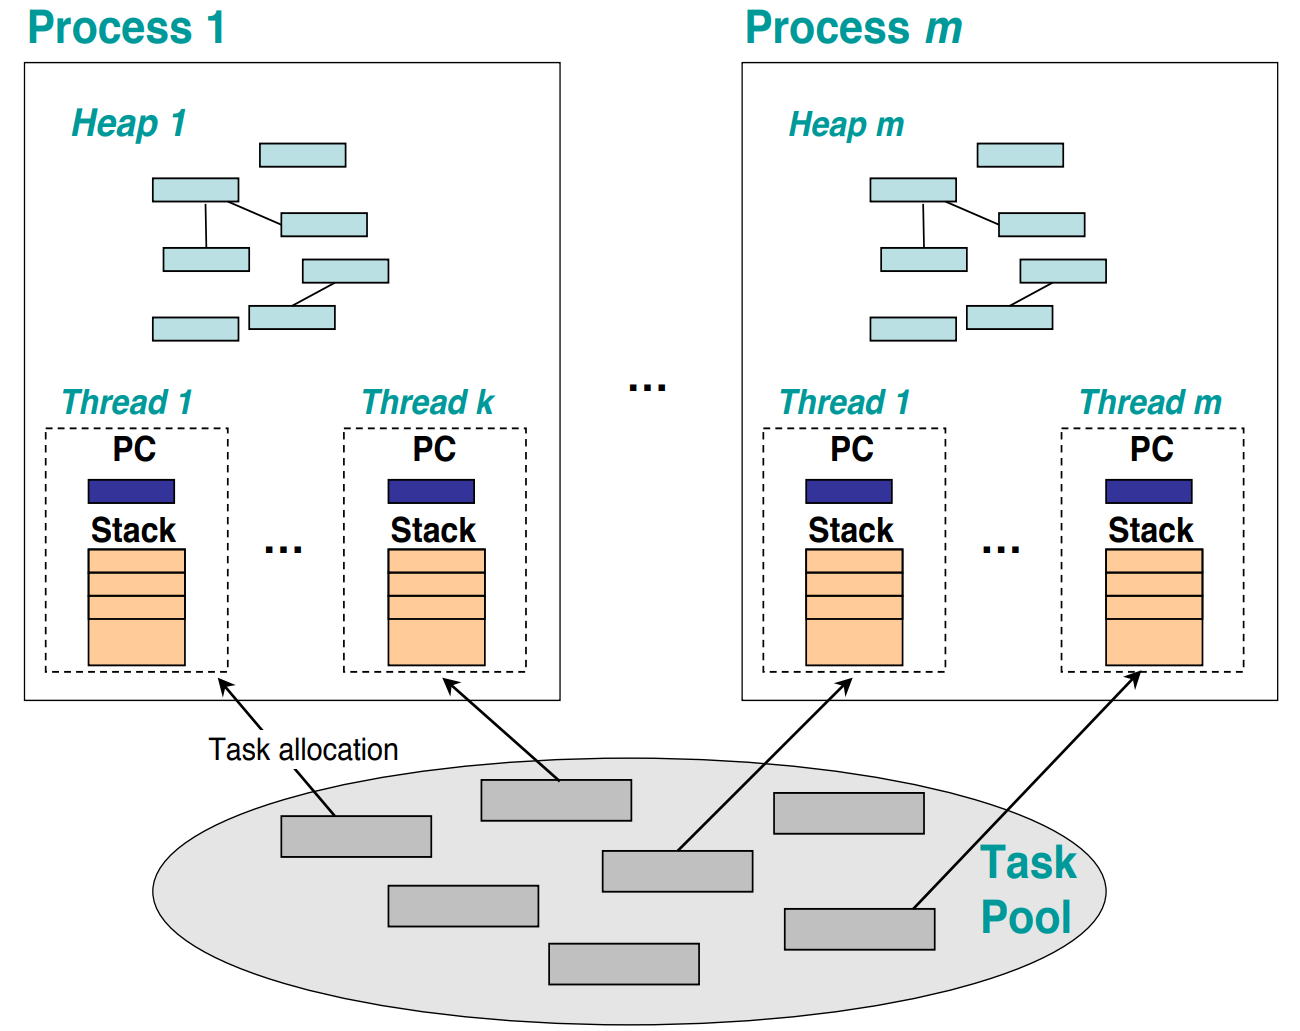
\includegraphics[width=0.6\textwidth, keepaspectratio]{imgs/terminology.png}
\caption{Diagram of how parallel processes are split up into threads and tasks.}
\end{figure}
\noindent
\textbf{Process} - A process is an independent unit of computation with private address space and usually comprises of multiple threads. The process-thread model does not include registers so it is not hardware-specific. 
\n
\textbf{Task} - Indicates a unit of computation that has been identified by the programmer, for example in a workpool setting and is often used synonymously with thread.
\n
\textbf{Thread} - The basic unit of parallel computation. It is lightweight and shares address space with other threads in the same process, but has its own separate stack and program counter. 
\n
\textbf{Filament} - Filaments wind together to form threads. These are primitive units of pure computation which does no communication. Filaments don't necessarily need context switching if they are small enough because they will terminate with a result. 

\subsection{Granularity}
Granularity is a \textbf{relative} measure of the ratio of the amount of computation to the amount of communication within a parallel algorithm implementation. In other words, it is a term used for the size of a parallel task in terms of its execution time. 
\n
For example, \textbf{coarse-grained} tasks are larger and relatively few in number while \textbf{fine-grained} tasks are smaller but in larger numbers. If a program is too coarse-grained, then there is not enough parallelism, resulting in poor utilisation. On the other hand if a program is too fine-grained, the overhead of thread creation and communication overtakes the benefit gained from parallel computation. A big issue in parallelism is determining the optimal granularity of a task.
\begin{figure}[H]
\centering
\begin{subfigure}{0.47\textwidth}
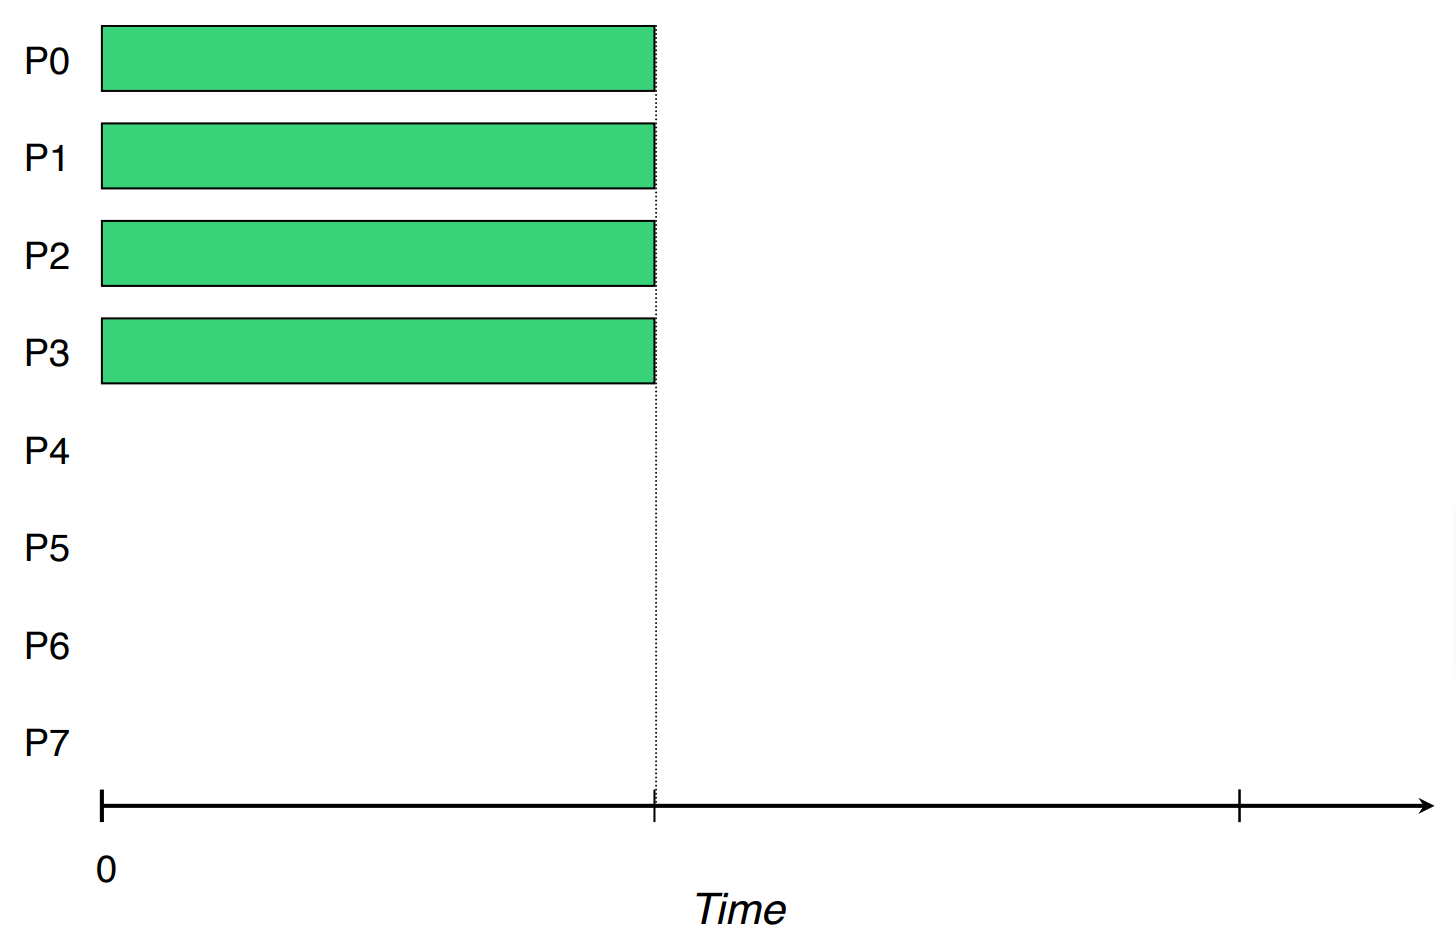
\includegraphics[width=1\textwidth, keepaspectratio]{imgs/granularity-little.png}
\caption{Too little granularity}
\end{subfigure}
\hspace*{\fill}
\begin{subfigure}{0.47\textwidth}
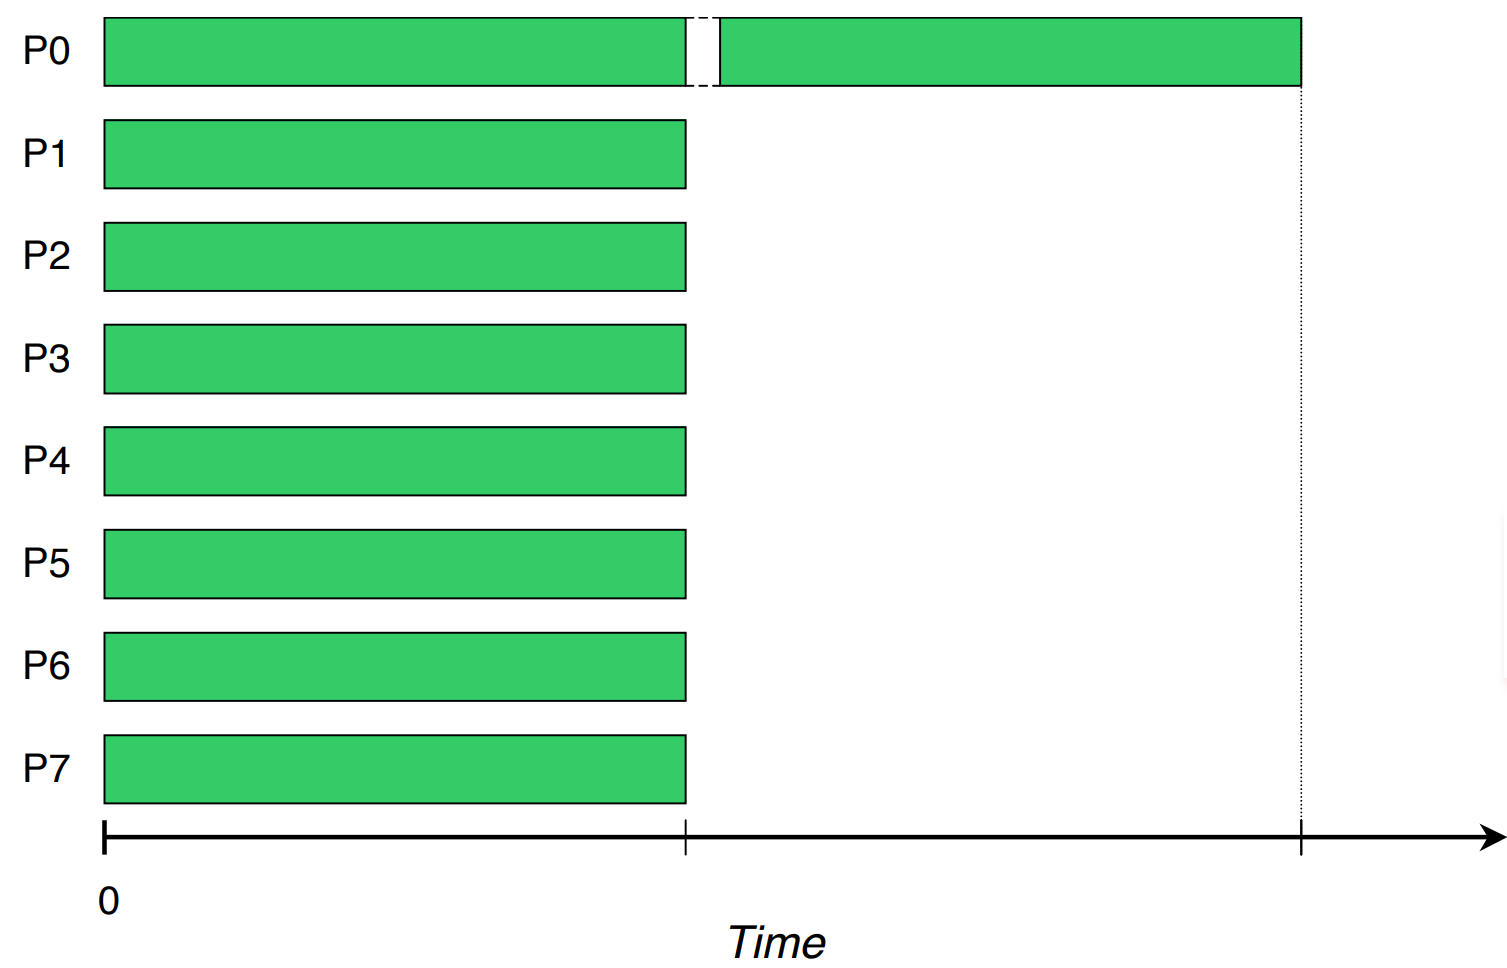
\includegraphics[width=1\textwidth, keepaspectratio]{imgs/granularity-much.png}
\caption{Too much granularity}
\end{subfigure}
\end{figure}
\noindent
The granularity is partially determined by three characteristics of the algorithm to parallelise and the hardware used to run the algorithm.
\begin{itemize}
\item \textbf{Structure of the problem} - Algorithms that are inherently \textit{data-parallel}, that is few unique operations are done over many pieces of data are often fine-grained by definition, as the same operation is applied to all the data. On the other hand, if only larger subroutines can be executed in parallel which require many calculations and little communication, then they are inherently coarse-grained. 
\item \textbf{Size of the problem} - Given 10 data elements and 10 processing elements (PEs), then only 1 clock cycle is required to process all 10 elements in parallel. However if the problem size is increased to 100 elements, then each PE now has to work on 10 elements each. This implies that larger sized tasks are more coarse-grained by default.
\item \textbf{Number of processors} - By the same token as the size of the problem, the number of processors also directly affects granularity as there are only so many limited processing units. More processors would lead to more fine-grained granularity as each processor has to do less, provided the size of the problem stayed constant. 
\end{itemize}
Granularity is important in choosing the most efficient paradigm of parallel hardware for the algorithm at hand. For example SIMD architectures are best for fine-grained algorithms while MIMD architectures are less effective due to the message-passing needed between MIMD cores. This further indicates that communication speed is a factor in choosing granularity, as a fine-grained task would be heavily hampered by slow communication while coarse-grained tasks would be effected less. 

\subsection{Amdahl's law}
Amdahl's law is a law which governs the speed-up of parallelism on a given problem. It is used as a way to determine limits on parallel optimisation. It states that 

\section{Parallel Haskell}



























\end{document}